\section{Komplexe Funktionen}
\subsection{Exponential-/Logarithmusfunktion}
\[e^{j\zeta}=\cos\zeta + j\sin\zeta\]
Realteil $z_1$ von $e^{z_1+jz_2}$ ist der Streckungsfaktor. Der Imaginärteil $z_2$ ist der zweite Term.

\subsection{Trigonometrie}
\[\sin(z) = \frac{e^{jz} -e^{-jz}}{2j} \qquad \cos(a) = \frac{e^{jz} +e^{-jz}}{2} \qquad (z \in \mathbb{C})\]

\subsection{Harmonische Schwingungen}
\todo{Summe von Komplexen Amplitude}

\subsection{Logarithmus und Potenzen}
$\mathbb{R}: \ln(1) = 0 \quad \mathbb{C}: \Ln(1)= 2k\pi j$
\[\Ln(z) = \ln(\left|z\right|) + j\cdot arg(z) \]
\todo{$\Ln(0)$ ndef!}

\subsection{Abbildungen}
Um eine Abbildung durch eine Funktion auszudrüken werden gegebene Komplexe Zahlen parameterisiert und mit der Funktion verrechnet.
\todo{KW 17 Di. Nachmittag\\
\[z = r + cj \rightarrow f(z) \rightarrow w \]
}

\subsection{Ableitung}
Wie in $\mathbb{R}$. Ableitung $f'$ entspricht jedoch einer Dreh-/Streckung mit Faktor $f'$. \textbf{Winkel} entspricht Ortsvektor zu Re-Achse von $f'$. Die \textbf{Streckung} ist der Betrag von $f'$.
\todo{Fr. 30.4.21}

\subsection{Potenzfunktion $z^n$}
\todo{}

\subsection{Kehrwertfunktion $\frac{1}{z}$}
\todo{% TODO: \usepackage{graphicx} required
	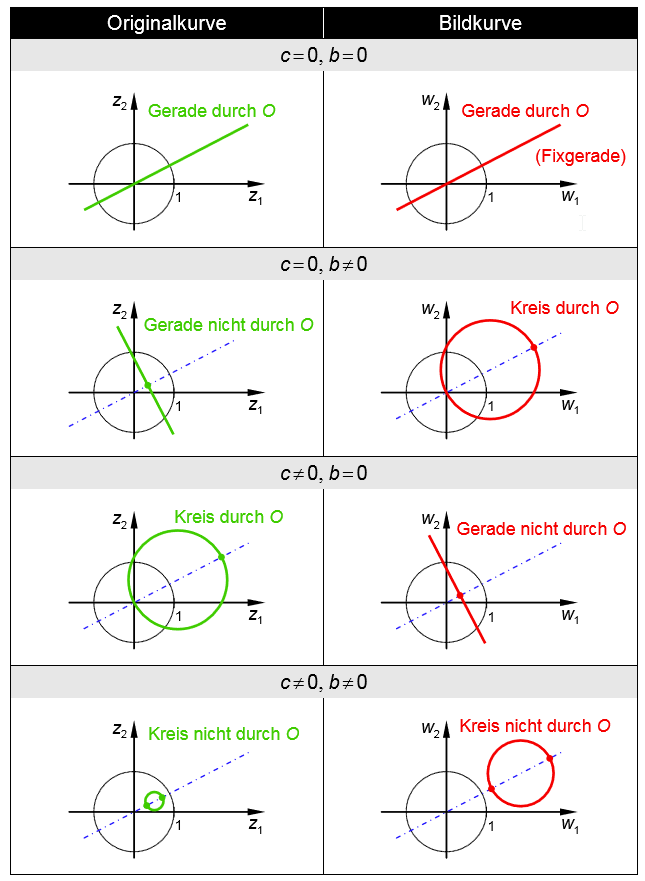
\includegraphics[width=\linewidth]{Images/screenshot007}
}
\todo{Fr 7.5.21}

\subsection{Möbiustransformation}
\todo{Di. 11.5.21 \\
	\[f(z) = \frac{az+b}{cz+d}\]
}

\subsection{Joukowski-Funktion}
\todo{Di. 11.5.21 \\
\[f(z) = z + \frac{1}{z}\]
}

\subsection{Exponentialfunktion-Funktion}
\todo{Di. 11.5.21 \\
	\[f(z) = e^z\]
}

\subsection{Trigo-Funktion}
\todo{Di. 11.5.21 \\
	\[f(z) = e^z\]
}